\section{Systematisk Test af Program}
\label{sec:systematisk_test_af_program}

\subsection{Test Driven Development}
\label{sub:test_driven_development}

For at sikre et program der er let at teste, er kernefunktionerne i programmet udviklet med metoden Test Driven Development. I Test Driven Development (TDD) skrives unit tests af en metode, umiddelbart før selve implementationen af funktionen. Denne metode sikrer, at en ny funktionalitet ikke ødelægger en allerede eksisterende funktionalitet \cite{martin2006agile}. Derudover tvinges programmøren til at tænke på, hvordan metoden bruges ved kald. Dermed sikres det at metoden er nem at kalde.

Et andet aspekt af TDD, er at testkoden er en form for dokumentation for den testede metode.

\subsection{Unit Testing i Microsoft Visual Studio}
\label{sub:unit_testing_i_microsoft_visual_studio}

Til unit testing er Microsofts unit test framework for managed code brugt. Frameworket kan teste managed code, som c\# falder ind under. Når tests er skrevet, kan Test Explorer i Visual Studio køre testene. Når testene er færdige, vil resultaterne blive præsenteret som failed tests, passed tests, not run tests og skipped tests \cite{msdn_unittest}.

\begin{lstlisting}[label=lst:test_notfound, caption={Eksempel på testfunktion}]
  [TestMethod]
  public void ShouldThrowWhenNotFound()
  {
      var space = new WaterSpace(404404, 4.3, 5.4);
      try
      {
          var test = BoatDetector.BoatAt(space);
      }
      catch (KeyNotFoundException _)
      {
          return;
      }
      Assert.Fail("No exception was thrown.");
  }
\end{lstlisting}

For at skrive unit tests, skal der oprettes et unit test projekt. Herefter kan der tilføjes klasser annoteret med \enquote{[TestClass]}. Inde i disse klasser, tilføjer man de metoder, annoteret med \enquote{[TestMethod]}, som skal køres. Et eksempel på en test metode, kan se i \cref{lst:test_notfound}. Alle tests til systemet kan findes på CD'en der afleveres som bilag.

\begin{figure}
  \centering
  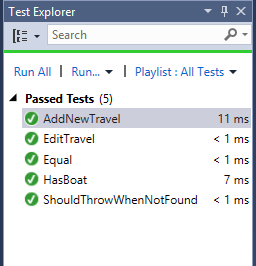
\includegraphics{test_explorer.png}
  \caption{Resultat af tests i Test Explorer i Visual Studio 2013}
  \label{fig:test_explorer}
\end{figure}
